\section{Physical Implementation}
\label{sec:PCB-implementation}

The final, delivered module is a $90mm\times62mm$ PCB. The PCB manufactured 
for the project was done so for free, using Spirit Circuits' "Go Naked"
service \cite{go-naked}. The PCB itself is a "tracks and holes" only service 
- no soldermask or silkscreen is applied. The schematic of the circuit 
delivered is available in Appendix ???, and of the PCB layout in Appendix 
???. A waterproof lacquer will be applied to the PCB to prevent condensation 
from shorting tracks together, and the module itself presented in a 
waterproof container before flight testing.

\begin{figure}[H]
        \centering
        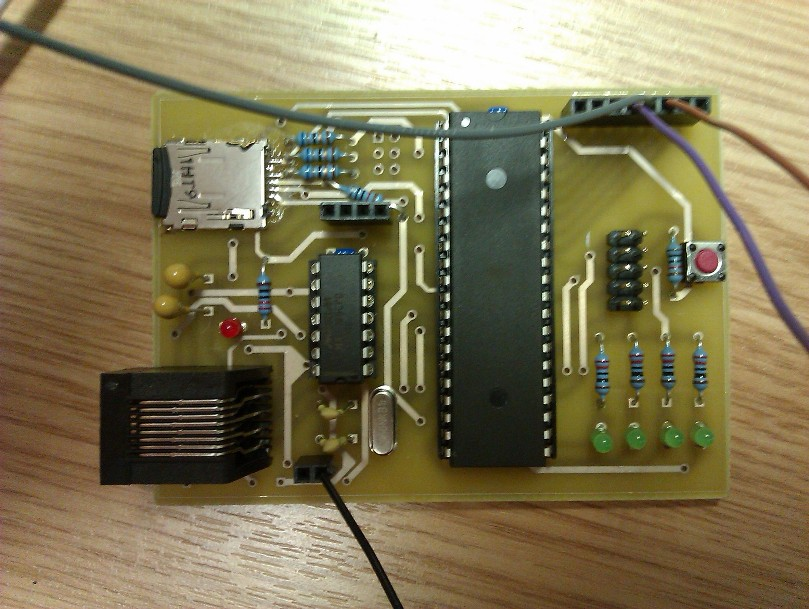
\includegraphics[width=1.00\textwidth]{figures/PayloadImplementation.jpg}
        \captionof{figure}{Image of the final payload, under test, before lacquer is applied. R11 can be seen between the Camera header and a via near the SD card Vcc}
        \label{fig:PayloadImplementation}
\end{figure}

Due to an issue discovered between ordering and receiving the PCB, an 
additional 10k$\Omega$ resistor has been placed between Camera RX and 3V3 (R11 
on the schematic). Also, the Single In Line header holes (for the Port A 
expansion and camera headers) have been widened from 0.40mm to 0.80mm. An 
update to the PCB layout is provided in the delivered repository.

The camera will also be presented in a sealed, weatherproof container.